\documentclass[a4paper,10pt]{article}
\usepackage[utf8]{inputenc}
\usepackage{charter}
\usepackage[english]{babel}
\usepackage{amsmath}
\usepackage{amsfonts}
\usepackage{graphicx}
\usepackage{caption}
\usepackage{float}
\usepackage{hyperref}
\usepackage{setspace}
\usepackage[top=2cm,bottom=2cm,left=3cm,right=2cm]{geometry}
\usepackage[usenames,dvipsnames]{xcolor}
\usepackage{setspace}
\usepackage{fixltx2e}     % to get subscript',
\usepackage[style=numeric,backend=biber]{biblatex}
\usepackage[acronym]{glossaries}
\usepackage{makeidx}
\usepackage{nomencl}      %Variable nomenclature
\usepackage{textcomp}
\usepackage{sfmath}
\usepackage{booktabs}     %to get bottomrule top rule and middlerun in tabular',
\usepackage{algorithm}
\usepackage{algorithmic}
\usepackage{rotating}

% \usepackage{fontspec}
% \setmainfont{Sora}[
%   Path = /usr/share/fonts/googlefonts/static/,
%   Extension = .ttf,
%   UprightFont = *-Regular,
%   BoldFont = *-Bold,
%   ItalicFont = *-Regular
% ]

% \newfontfamily\italicfont{Sora}[
%   Path = /usr/share/fonts/googlefonts/static/,
%   Extension = .ttf,
%   UprightFont = *-Regular,
%   FakeSlant = 0.2
% ]

% \DeclareTextFontCommand{\textit}{\italicfont}


% parameters
\newcommand{\parametertype}[5]{
\begin{center}
\begin{tabular}[c]{|c|c|c|c|c|}
\hline Type & Default value & Min & Max & Min Resolution \\
\hline #1 & #2 & #3 & #4 & #5\\
\hline
\end{tabular}
\end{center}
}

\newcommand{\parametercolor}[1]{{\color{blue}{#1}}}

\newcommand{\parameter}[1]{\parametercolor{\gls{#1}}}

\newcommand{\newparameter}[3]{
\newglossaryentry{#1}{
  type=parameters,
  name={#2},
  description={#3}
}
}
% usecases
\newcommand{\usecase}[3]{
\textbf{Usecase:} #1 \\
{\small ID: #2} \\
#3 \\}

% system requirements
\newcommand{\sysreq}[3]{
\textbf{Sys-Req:} #1 \\
{\small ID: #2} \\
\textbf{Rationale: }#3\\}


\include{acronym_glossary.tex}

\newglossary[plg]{parameters}{pmt}{ptn}{List of Parameters}

\newparameter{aebsafetydistance}{aeb\_safety\_distance}{Minimum, safety distance between ego and target once the ego is stopped
\parametertype{Float}{3.0}{0.0}{10.0}{0.1}}

\newparameter{warningduration}{fcw\_warning\_duration}{Duration of audio warning prior to the \gls{AEB} enagement
\parametertype{Float}{0.9}{0.0}{5.0}{0.1}}


\usepackage{titlesec}
\titleformat{\part}[block]
  {\normalfont\bfseries\Huge}{\thepart}{1em}{\Huge}

\titleformat{\chapter}[block]
  {\normalfont\bfseries\Huge}{\thechapter}{1em}{\Huge}



\title{Requirements}
\author{Maxime Haselbauer}
\addbibresource{./library.bib} %define so to work with mendeley',
\setlength{\parindent}{0pt}                % Avoid indentation on the first line',
\makeindex
\makenomenclature
\makeglossaries

\begin{document}
\maketitle
\begin{abstract}
Set of requirments for a simple STM32 hello world project
\end{abstract}
\printnomenclature
\printglossaries


\nomenclature{$a$}{The variable a}

\section{Use cases}
\usecase{Destkop client stays alive if device not connected}{001}{The desktop application is launched by there is no device connected. It stays on and wait until a device is connected.}

\begin{figure}[ht]
	\centering
	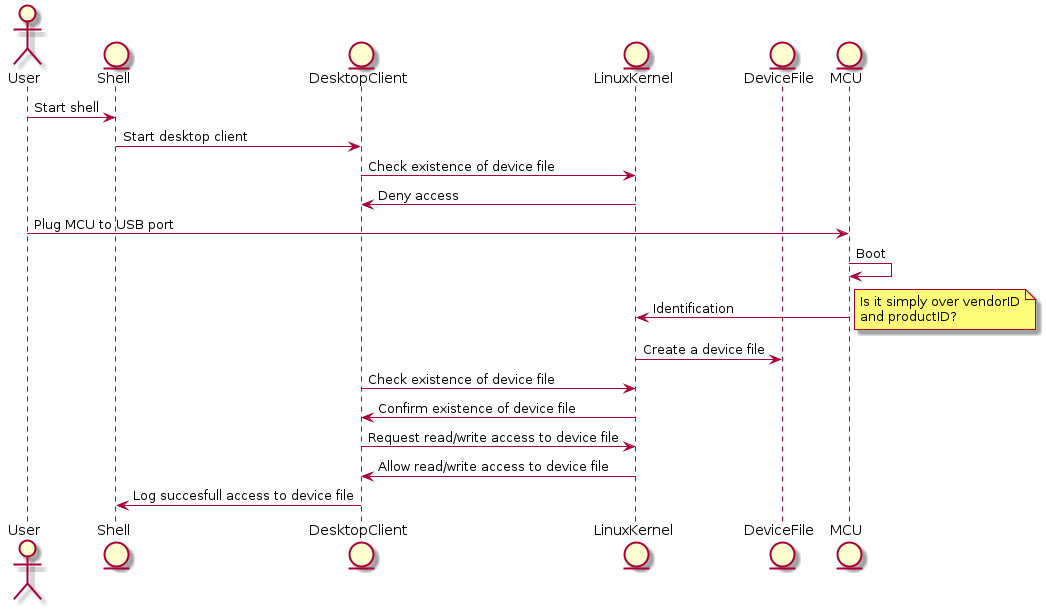
\includegraphics[width=1.0 \textwidth]{./diagrams/pc_mcu_interaction_diagram.png}
	\caption{PC-MCU interaction diagram}
	\label{fig_pc_mcu_interaction}
\end{figure}

out


\section{The first section}
\newacronym[longplural={First Acronyms}]{FAlabel}{FA}{First Acronym}
This is how to use the \gls{FAlabel}. And now making a second use of \gls{FAlabel}.
\cite{fooAuthor}

\begin{figure}[ht]
	\centering
	
\includegraphics[width=0.75 \textwidth]{../resources/project_logo.png}
	\caption{caption}
	\label{reference}
\end{figure}

The first equation is referenced as \ref{eq:eqFirstequation}.
\begin{equation}
S~=~\Pi R^2
\label{eq:eqFirstequation}
\end{equation}

\printbibliography
\end{document}
